\input{chapter-header.tex}
% =============================================================================
\chapter{Introduction}
\chaplabel{introduction}
\minitoc
% =============================================================================


%Reflective systems are those that reason about and act upon themselves \cite{Smit84a}. A causal connection exists between the program and its representation inside the program itself as a meta-program \cite{Maes87a}. This reflective architecture introduces self-references:  an object-oriented system is composed by objects, which are instances of classes, which are also objects, and so on. These self-references, also known as meta-circularities \cite{Chib96a}, allow the manipulation of several meta-levels on one infrastructure.
%
%Reflective systems traditionally modify their self-representation to evolve and define new abstractions. However, the self-modification approach of evolution has many drawbacks, such as making difficult the self-surgery operations~\cite{Casa09a} or the lose of the reproducibility of the system. On the other hand, non-reflective systems develop an evolution approach by recreation. Whenever a change has to be made to the system, a new system is created with the new changes applied. This approach solves many of the drawbacks of the reflective approach.
%
%\gp{add some sentences on why it is important to evolve, which kind of software artifacts we would like to evolve, why it is challenging}

% =============================================================================
%\section{The need for Software Evolution}
% =============================================================================

Software inevitable changes and we need to provide with the tools and methodologies that support such changes~\cite{Nier08b}. However, production-ready applications are not usually change-aware. These applications should be either engineered from scratch with change in mind, or a lot of reengineering effort should be invested in them to support change. Making deep modifications to a language runtime can be a cumbersome task.
In the last years, evolving a language runtime has become an important task. Multicore hardware brought new problems on concurrency and parallelism; the \emph{cloud} increased the need for software adaptation; new resource constrained devices presenting new challenges to software developers. The software we use, and in particular the programming languages and tools we use should be easily tailorable to support many of the new challenges that come with new technology and needs.

% =============================================================================
%\section{Resource Constrained Devices}
% =============================================================================

%\gp{noury had a reference on this -> everything is going small}

%Unused deployed code units have an undesired impact when targeting a constrained infrastructure. 
%Constrained devices may present restrictive hardware such as low primary or secondary memory, or even software impositions such as the Android's Dalvik VM restriction to deploy only 65536 methods\footnote{According to dalvik's bytecode documentation~(\url{http://source.android.com/devices/tech/dalvik/dalvik-bytecode.html}), the source register accepts values between 0 and 65536.}. Big JavaScript mashup applications have an impact on loading time due to network speed and parsing time.
%These limitations may forbid the deployment of applications that contain lots of code units, or limit the amount of applications and content an user can have in its device.

%Existing solutions to this problem propose the extraction of used code units of an application to reduce their size and memory footprint. Java Micro Edition~\cite{JavaME} proposes a general purpose specialized runtime environment with no possibility of customization. Other solutions in the field propose to automatically detect and extract used code units, so called \emph{tailoring}, with static call graph construction as the most dominant technique~\cite{ShortGrov97a}. 
%Static approaches present limitations in the presence of dynamic features such as reflection or in the absence of static type annotations. Additionally, these existing solutions are generally designed to extract all used code units with no possibility for the user to customize the process of selection.

For example, an application runtime should be easily tailorable to consume less resources. We can observe that deployed applications contain a set of \emph{code units} such as classes and methods that tend to occupy more memory~(primary and secondary) than necessary.
%Besides, an application may load a code unit that is only partially used, such as a class with some methods that are never invoked.
%Deployed object-oriented applications often contain \emph{code units}~(e.g. packages, classes, methods) that the running application never uses. 
This problem shows itself more evident and harder to control under the usage of third party software. 
Third party libraries and frameworks are designed in a generic fashion that allows multiple usages and functionalities, while applications use only few of them. 
Examples are logging libraries, web application frameworks or object-relational mappers.


%Figure~\ref{fig:unusedCodeUnits} shows a typical deployment scenario with unused code units.
%
%This problem becomes more evident with the inclusion of third party libraries~(and frameworks). 
%Third party libraries provide often a great variety of code units, usually designed in a generic fashion. 
%They allow multiple usages, while applications tend to use only some of them. 
%Additionally, application developers do not often modify and customize third party libraries to fit their needs but use them as black boxes. 
%Modifying them would mean to lose compatibility with the original development branch of the library and having deep knowledge on the library.
%
%\begin{figure}[ht]
%\begin{center}
%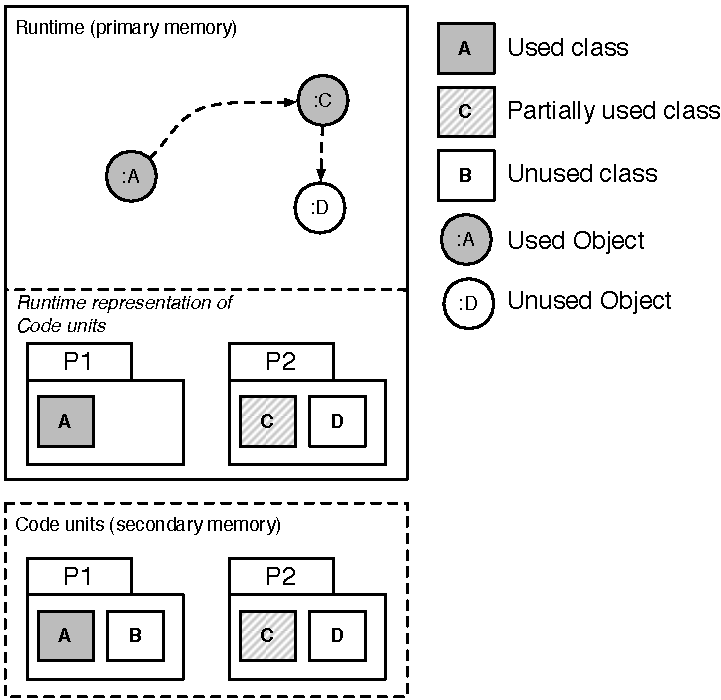
\includegraphics[width=1\linewidth]{components}
%\caption{\textbf{Unused Code Units.} Package P1 contains class A which is used during runtime and class B which is never needed and thus, not loaded. Package P2 contains class C which is partially used~(it contains methods that are never invoked) though it's completely loaded. Class D is loaded because an instance of it is created, but it is never used.\label{fig:unusedCodeUnits}}
%\end{center}
%\end{figure}

Unused code units represent serious drawbacks in constrained devices. 
First, unused code units may forbid the deployment into a constrained resource device.
It may also interfere with the deployment and usage of other applications, because of large memory footprints in both secondary~(disk storage) and primary~(RAM) memory~\cite{Mart12a} or the presence of slow networks in the case of rich web applications.
Second, some deployment targets may have an infrastructure designed in such a manner that forbids the deployment of large applications. For example, the Android's Dalvik VM restricts an application to deploy only 65536 methods.


% =============================================================================
%\section{The cloud and Mobile code}
% =============================================================================

%\gp{explain why code mobility is important!}

Another example of support that should be brought to user applications is \emph{code mobility}. Code mobility is a mechanism that allows the migration of programs between different environments. This problem is important in the context of ubiquitous systems and virtualization technology. Code mobility provides support for \eg load balancing, adjusting an application's resources dynamically and functionality customization. Fuggetta et al. define informally code mobility as the capability to rebind a piece of code with the location it is running~\cite{Fugg98a}. Such rebinding may consist, depending on the style of mobility, in the mobility of execution state, application data and resources, or both of them. Execution state mobility is the ability to suspend the actual execution of a program and transfer its internal execution information~(\eg code, execution stacks, instruction pointers) to some other environment. Data mobility is the ability to transfer the application's data~(\eg objects, database connections, files) between different environments.


% =============================================================================
\section{What to Evolve?}
% =============================================================================

High-level language runtimes are inherent complex pieces of software.
First, high-level languages virtual machines~(\VMs) have to combine two rather extreme goals: abstraction and performance.
We have seen that the required abstraction for the running high-level language has a strong influence on the \VM design.
At the same time the hard performance requirement requires precise interaction with the underlying hardware.
This goes even so far that specialized hardware is conceived to match the performance requirements \cite{Unga84a,Stef84a,McGh98a,Clic05a}.


We run our languages and applications on top of these complex \VMs.
Then, our programs must comply to the contract required by the \VM to run, namely the \VM's \emph{execution model}.
A \VM's execution model imposes for example an object format, a class or prototype model to perform a method lookup, a bytecode set to execute methods at runtime.
In some cases, the \VM also loads and initializes the language structures.
These \VM-language complex interactions makes difficult to evolve any of these elements without affecting the other.

In the following sections we propose a dissection of a high-level program. We made this dissection with the objective of understanding the relation and separation between the elements we believe important in the context of software and language evolution. The identified elements will also serve for the understanding of the rest of this dissertation. Figure \ref{fig:whatToEvolve} shows an schema of this dissection.

\begin{figure}[!ht]
\begin{center}
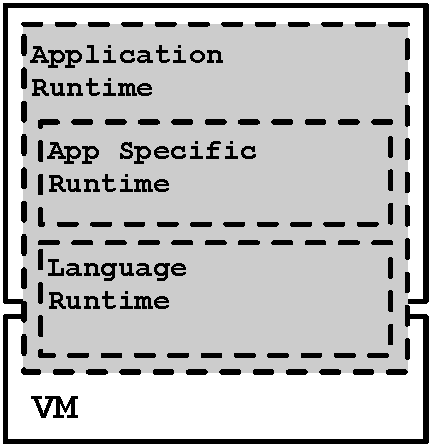
\includegraphics[width=0.6\linewidth]{elements_to_evolve}
\caption{\textbf{What to Evolve.}\label{fig:whatToEvolve}}
\end{center}
\end{figure}



\subsection{Virtual Machines}

\VMs concentrate several complex and interconnected elements with two main purposes: first it is to abstract applications from details such as memory management or machine specifics; second is to do that while also obtaining good performance.
The early \VMs focused on interpreting an abstract instruction set (bytecodes).
The benefits are twofold.
On the one hand the bytecodes guarantee certain platform independence by abstracting away from the \CPU specific instruction set.
On the other hand bytecodes allow to encode complex operations into little space both serving the hard memory constraints of the hardware and simplifying the design of a compiler.
Obviously this abstraction gain comes at a cost and ever since the first \VMs were built research and industry strive to reduce the interpretation overhead.
An efficient way to improve performance is to use a just in time compiler (\JIT) that dynamically generates native code from the bytecode \cite{Deut84a}.
In this case the bytecode becomes an intermediate representation (\IR) for a bigger compiler infrastructure.
However, \JIT compilers are notoriously complex as they crosscut many \VM components.
At the same time they crosscut all abstraction layers; they have to access high-level information from the running bytecodes and manage native code at the same time.
Similar complexity applies to the automatic memory management present in most high-level language \VMs.
Garbage Collectors (\GC) evolved from simple helpers to complex software artifacts that for instance support concurrent garbage collection \cite{Clic05a}.

In this context, being able to evolve a \VM is crucial for language evolution, as \VMs are the enablers of many of the features in programming languages. A \VM complexity should be engineered to favor its change. In this thesis we do not focus on \VM evolution but on the languages and applications that run of top of them and their models. Although \VMs are very interlaced with the languages we want to evolve since they impose and constraint our languages to their execution model.

\subsection{Application Runtime}

The application runtime is the set of elements that an application includes at runtime \eg libraries, objects, classes, methods. The \VM interprets and executes the application runtime. Indeed, with this purpose the application runtime must comply to the \VM execution model~(Figure \ref{fig:whatToEvolve}).

The \emph{language runtime} is the subset of the application runtime that describe the language concepts and behavior \ie the set of classes and methods that describe the language internals. This language runtime concretizes the model that the language proposes to the developers. For example, Pharo Smalltalk proposes a programming model of classes with metaclasses~(the class of a class). This programming model is implemented in the language with also the concrete existence of the \ct{Class} and \ct{Metaclass} classes. This language runtime is not only composed by classes but also by other objects and elements. For example, it contains a table of interned strings or \emph{symbols} that should be guaranteed unique in the system.

While indeed an application runtime~(and therefore its language runtime) is coupled to its \VM to run, sometimes it is also coupled in its definition. That is, the \VM defines and fixes the language model and some of the initially loaded libraries. In this context, we focus on the evolution of application runtimes. Changing a language runtime is a way of extending and/or specializing the concepts provided by the language. These manipulations could also be applied in application runtimes as a whole. However, we should apply such modifications while still comply to the execution model of the \VM.


% =============================================================================
%\section{Problem Statement}
% =============================================================================

\section{Problems Modifying a Language Runtime} \label{sec:bootstrapping_problems}

We identify three main limitations when we aim to change a language runtime. First, how flexible a language definition is to be changed and adapted. Second, the unclear mixture of \VM and language concerns prevents us to extract the language definition and easily replace it. Finally, the differences in the abstraction levels and tool support between the language we are building and the language we use to build it makes it a challenging task.


\subsection{Flexibility to Change a Language Runtime}

The \VM is often the component in charge of initialising the language runtime. This decision is indeed practical as the \VM can safely initialise the language structures and solve the language bootstrapping issues avoiding recursions~\cite{Kicz91a}~(\eg create the first class without a class). This language runtime must comply at runtime to the execution model imposed by the \VM~(\eg an object format denoting how objects are represented in memory and a set of instructions for execution such as bytecode or assembly). This coupling is indeed necessary to run a program but does often remain hidden in hardcoded assumptions.

\begin{figure}[ht!]
\begin{code}
void Init_class_hierarchy(void) {
    rb_cBasicObject = boot_defclass("BasicObject", 0);
    rb_cObject = boot_defclass("Object", rb_cBasicObject);
    rb_cModule = boot_defclass("Module", rb_cObject);
    rb_cClass =  boot_defclass("Class",  rb_cModule);

    rb_const_set(rb_cObject, rb_intern("BasicObject"),rb_cBasicObject);
    RBASIC_SET_CLASS(rb_cClass, rb_cClass);
    RBASIC_SET_CLASS(rb_cModule, rb_cClass);
    RBASIC_SET_CLASS(rb_cObject, rb_cClass);
    RBASIC_SET_CLASS(rb_cBasicObject, rb_cClass);
}
\end{code}
\caption{\textbf{Code of the Ruby VM that initialises the class hierarchy (excerpt).} The VM code fixes the language class hierarchy.\label{code:ruby_hierarchy}}
\end{figure}

These hardcoded \VM assumptions have two main consequences when we target to change the language runtime: the \VM fixes its initial structures~(\eg Ruby's class hierarchy in Figure \ref{code:ruby_hierarchy}) and they introduce code duplications to manipulate language objects.
To illustrate this second problem, let us consider the code in Figure~\ref{code:logic_dup} that creates a \ct{Dictionary} or hashmap. A language runtime that is defined by a \ct{Dictionary} object to keep \eg a map of global objects, must execute the code in the figure to create the corresponding instance. However, since the language runtime and the \VM are in middle of their initialization, the \VM cannot execute this code as it is, and thus it cannot enforce its own invariants. The state of the art \VMs will provide an alternative low-level representation of the same code respecting the same invariants~(Figure~\ref{code:logic_dup2}). This introduces a redundancy: the \VM and the language have different code to honor the same invariants.

\begin{figure}[ht]
\begin{code}
Dictionary class>>new: n
    ^ self new initialize: n

Dictionary>>initialize: n
    "Initialize array to an array size of n"
    array := Array new: n.
    tally := 0
\end{code}
\caption{\textbf{Code to create a \ct{Dictionary} object in Smalltalk.}\label{code:logic_dup}}
\end{figure}

\begin{figure}[ht]
\begin{code}
void* createDictionaryWithSize(int n){
    void* dictionary, internalArray;
    dictionary = instantiateClass("Dictionary");
    internalArray := instantiateClass("Array", n);
    setInstanceVariable(dictionary, 1, internalArray);
    setInstanceVariableInt(dictionary, 2, 0);
    return dictionary;
}
\end{code}
\caption{\textbf{Code to create the same \ct{Dictionary} object from C.}\label{code:logic_dup2}}
\end{figure}


%This execution model is often less restrictive than the object models of the language's that run on top of them. For example, the Smalltalk and Ruby \VMs require for each object in the system to have a class, and each class a superclass, but there is no need for metaclasses.

After the language initialization, reflective languages~\cite{Smit84a} such as LISP or Smalltalk provide the means to modify themselves at runtime. These languages are based on a reflective architecture presenting the notion of causal connection~\cite{Maes87a}: a link between a programming element and its representation that keeps both in synchronization. However, as these languages contain meta-circular definitions in their kernel~\cite{Chib96a}, this can result in a Metastability problem~\cite{Kicz91a} \ie a change in the language runtime may introduce a meta-call recursion and turn the system unusable.% In this context, Reflectivity~\cite{Denk08b} is a framework that scopes reflection to avoid meta-call recursions.  Reflectivity succeeds to control behavioural reflection by accounting the level of \emph{metaness} of the execution in a program and executing reflective operations when it is in the correct meta-level. The main limitation of Reflectivity is that it does not allow structural reflective changes in the language runtime.

Finally, snapshot-based languages offer different means to evolve a language runtime. Instead of being reinitialized each time we need it, the state of the whole graph of objects that denotes the running program can be suspended and saved as a snapshot in a file. Later on, the program in this snapshot can be restarted from the point it was suspended. As a consequence of this persistency property, some snapshot-based languages such as Squeak or Pharo  do not have the infrastructure to be reinitialised from scratch. Indeed, their current deliverable snapshots are the result of a chain of side effects (updates and migrations) made to the original Smalltalk-80 snapshot. Thus, even if we can change the language runtime at runtime, they cannot ensure a reproducible initial state for their users.

\subsection{Mixture of \VM and Language Concerns}

The unclear interface between the language and the \VM makes difficult to recognize whether a piece of code belongs to a \VM or language concern. This causes undesirable temporal couplings between these two elements and prevents us to clearly extract and replace the language definition by another one.
To illustrate this problem, Figure \ref{code:jikes_vm_initialization} shows an excerpt of the JikesRVM\footnote{Taken from the version 3.1.3 of the JikesRVM in \url{http://sourceforge.net/projects/jikesrvm}}~\cite{Alpe00a}. In this example, the memory manager is initialised in the middle of the initial class loading phase. These memory manager calls are indeed needed to avoid the collection of objects during the initialization. However, it is necessary to call it after some specific classes are initialized and not before.

\begin{figure}[ht]
\begin{code}
private static void finishBooting() {
    ...
    MemoryManager.postBoot(); //Memory management
    ...
    runClassInitializer("java.lang.Runtime");
    runClassInitializer("java.lang.System");
    runClassInitializer("sun.misc.Unsafe");
    ...
    MemoryManager.fullyBootedVM(); //Memory management
    ...
    runClassInitializer("java.util.logging.Level");
    runClassInitializer("gnu.java.nio.charset.EncodingHelper");
}
\end{code}
\caption{\textbf{Code of the JikesRVM that initialises loads the initial classes of the runtime (excerpt).} The code performing the initial class loading is mixed with the code that initialises the memory manager of the \VM.\label{code:jikes_vm_initialization}}
\end{figure}

Snapshot-based languages, on the other side, show that language initialization and \VM initialization can be orthogonal. Indeed, languages such as Pharo, LISP or the V8 flavor of Javascript can restart their system from a snapshot. The \VM loads atomically the snapshot and binds it to the current runtime. Loading a snapshot clarifies the \VM startup steps as it replaces the phase of language initialization. Moreover, as long as the snapshot satisfies the \VM execution model, it can run any language model, as it is the case of Pharo and Newspeak that run on the same \VM.

%Other snapshot-based languages such as GNU-Smalltalk or the V8 flavor of Javascript possess both mechanisms: they recreate the language runtime from scratch, and can also restart from a snapshot. In the case of V8, the snapshot was chosen with performance in mind, to avoid parsing and recreation on client-side machines.

%\item[The \VM-Language interface is unclear.]
%For example, the \VM assumes how objects are structured in the runtime to manipulate them: the amount and size of their instance variables, object headers, special kind of object references~(\eg weak references). The \VM also needs access to some well-known objects to run code: this is the case for example of \ct{nil}, \ct{true} and \ct{false} objects. Another example of a tight coupling are the callbacks \VM-language, where the \VM can trigger some specific code on the language to notify it from some event.

\subsection{Abstraction Level and Tool Support}

On one side, when defining the language runtime at the \VM level, we rely on the tools and abstractions available to develop the \VM to change the language. That means that the language developer uses low-level abstractions to express higher-level concerns. This \emph{mismatch} impacts in the vm/language developer efficiency, as the tools it has are not adequate for the task it tries to accomplish. This problem is indeed aggravated with the complexity of such pieces of software, include elements such as the \GC or the JIT that cross-cuts every \VM concern. Indeed the developer would benefit from the productivity that a high-level language brings.

%To attack these problems, many programming systems have found desirable to follow the principles of \emph{high-level low-level programming} \ie expressing low-level concerns using high-level languages~\cite{Fram09a}. High-level low-level programming pursues the objective of simplifying the complexity of programming systems. By using a high-level language to describe the low-level world the developer benefits from their abstraction power and tooling of the first one. A clear example of this fact is the metacircular \VM field, where many projects whose goal is to write \VMs in a high-level language have blossomed in the last years~\cite{Wimm13a,Alpe00a,Verw11a,Inga97a,Unga05a,Rigo06a}. These projects are biased to \VM building techniques and not to the initialization of the languages that run on top of them.

On the other side, we found that reflective languages support naturally the usage of the language abstractions and tools to modify the language runtime. Reflective languages benefit from the reification of the language concepts to be able to change them from the language itself. Languages such as Smalltalk show how debuggers and code browsers can be built using such features.


\subsection{Problem Statement}

\gp{write from scratch}
A better language runtime initialization solution should have the following properties:
\begin{itemize}
\item Allow one to easily change the structure and behavior of the language runtime.
\item Clarify the separation between \VM and language.
\item Ensure the initial state of the language even in presence of a reflective architecture (Solving the bootstrapping and metastability problems as defined in AMOP~\cite{Kicz91a}).
\end{itemize}

% =============================================================================
\section{Thesis Outline}
% =============================================================================
%\sm{This dissertation structure is different to what I am used to. At least the way you announce the purpose of the chapters is not what I would expect.
%In my diss, everything revolves around one thesis, here, it is a number of things listed one after another, don't see the central motive I would expect}

\gp{write from scratch, left for the end}
\begin{description}
\item[\chapref{background}] sheds light on the context of this work.
	We present a quick overview of language-side reflection followed by a development of \VM-level reflection.
	We find that mostly metacircular \VMs provide limited \VM-level reflection and thus we present several high-level language \VMs falling into this category.
	We conclude that there is only two research \VM that has a uniform model for \VM and language-side.
	Among them is \P a research \ST \VM we contributed to previous to working on this dissertation.

%\item[\chapref{reification}] focuses on language-side applications that simplify the interaction with the underlying \VM.
%	We present a custom inspector framework that is now used by default in \PH.
%	As a second part we explain how we introduced first-class layouts and slots to \PH to reify the low-level structural layout of objects.
%	Both projects are crucial for metacircular \VM development and are direct results from the research conducted on the \P \VM.

\item[\chapref{benzo}] describes a high-level low-level programming framework named \B.
	The core functionality of \B is to dynamically execute native-code generated at language-side.
	\B allows us to hoist typical \VM plugins to the language-side.
	Furthermore we show how code caching makes \B efficient and users essentially only pay a one-time overhead for generating the native code.
	
\item[\chapref{ffi}] presents \NB, a stable foreign function interface (\FFI) implementation that is entirely written at language-side using \B.
	\NB is a real-world validation of \B as it combines both language-side flexibility with \VM-level performance.
	We show in detail how \NB outperforms other existing \FFI solutions on \PH.

\item[\chapref{validation}] focuses on two further \B applications.
	In the first part we present \WF a framework for dynamically generating primitives at runtime.
	\WF extends the concept of metacircularity to the running language by reusing the same sources for dynamic primitives that were previously used to generate the static \VM artifact.
	In a first validation we show how \WF outperforms other reflective language-side solutions to instrument primitives.
	
	In a second part of \chapref{validation} we present \NBJ a prototype \JIT compiler that is based on \B.
	\NBJ shows the limitations of the \B approach as it required a customized \VM to communicate with the existing \JIT interface for native code.
	Our prototype implementation generates the same native code as the existing \VM-level \JIT, however, it is currently limited to simple expressions.
	\NBJ shows that for certain applications a well-define interface with the low-level components of the \VM is required.

\item[\chapref{future}] summarizes the limitations of \B and its application.
Furthermore we list undergoing efforts on the \B infrastructure and future work.

\item[\chapref{conclusion}] concludes the dissertation.

\end{description}

% =============================================================================
\input{chapter-footer.tex}
% =============================================================================